 \documentclass{article}

%% Compile this with
%% R> library(pgfSweave)
%% R> pgfSweave
%\usepackage[nogin]{Sweave} %way to understand R code
\usepackage{pgf} 

%look it up
\usepackage{tikz} 

% allows R code or other stuff in the figure labels
\usepackage{subfigure} 

% allows to have subfigures
\usepackage{color} 

%colored text!
\usepackage[left=1.in,right=1.in,top=1.in,bottom=1.in]{geometry} 

% sets the margins
\usepackage{fancyhdr} 
\usepackage{setspace} 
\usepackage{indentfirst} 
\usepackage{titlesec} 
\usepackage{natbib} 
\usepackage{sectsty}
\usepackage{listings}
\usepackage[section]{placeins}

\usepackage{amssymb}
\usepackage{amsmath}
\usepackage{amsfonts}
\usepackage{float}
\usepackage[hyphens]{url}

\usepackage{lmodern}
\usepackage[T1]{fontenc}
\usepackage{textcomp}

\usepackage{blindtext}


\newcommand{\lang}{\textsf} 

%
\newcommand{\code}{\texttt} 
\newcommand{\pkg}{\texttt} 
\newcommand{\ques}[1]{{\bf\large#1}} 
\newcommand{\eb}{\\
\nonumber} 


%% The following is used for tables of equations.
\newcounter{saveEq} 
\def\putEq{\setcounter{saveEq}{\value{equation}}} 
\def\getEq{\setcounter{equation}{\value{saveEq}}} 
\def 
\tableEq{ 

% equations in tables
\putEq \setcounter{equation}{0} 
\renewcommand{\theequation}{T\arabic{table}.\arabic{equation}} \vspace{-5mm} } 
\expandafter\def\expandafter\UrlBreaks\expandafter{\UrlBreaks%  save the current one
  \do\a\do\b\do\c\do\d\do\e\do\f\do\g\do\h\do\i\do\j%
  \do\k\do\l\do\m\do\n\do\o\do\p\do\q\do\r\do\s\do\t%
  \do\u\do\v\do\w\do\x\do\y\do\z\do\A\do\B\do\C\do\D%
  \do\E\do\F\do\G\do\H\do\I\do\J\do\K\do\L\do\M\do\N%
  \do\O\do\P\do\Q\do\R\do\S\do\T\do\U\do\V\do\W\do\X%
  \do\Y\do\Z}


\def\normalEq{ 

% renew normal equations
\getEq 
\renewcommand{\theequation}{\arabic{section}.\arabic{equation}}}
\newcommand{\normal}[2]{\ensuremath{N(#1,#2)}}


\doublespacing 


\title{Ricker spawner-recruitment model fits for Harrison and Cowichan chinook salmon populations} 
\author{Catarina Wor} 



%\pgfrealjobname{pgfSweave-vignette}
%pgfSweave-vignette
\begin{document}
\maketitle

\tableofcontents

\section{Background}


The goal of this document is to examine spawner-recruitment dynamics for Harrison and Cowichan Chinook Salmon populations. We fit a various forms of the Ricker curve in order to examine potential parameter trajectories for the alpha and beta parameters. 


\section{Models}

We considered a set of eight estimation models that represent alternative forms of either time-invariant or time-varying stock-recruitment dynamics. All these models are based on the Ricker spawner-recruitment curve and include: stationary versions with and without auto-correlation in residuals, three versions with time-varying parameters described bya random walk (RWa, RWb, RWab). and three versions of regime shift models described by a hidden markov structure (Shift a, Shift b and Shift ab). For the purpose of this summary we ommit further description of the methods, but more details, including the R package used and detailed methods write-up are available upon request. 

We present results from model selection criteria for completeness. However, our preliminary research finds indicate that commonly used model selection criteria are often mislead in selecting the true underlying dynamics of the resource. We found that AIC and BIC tend to favour time-varying dyamics. Whereas cross-valiation methods, such as leave-future-out (LFO) tend to favour stationary model. 


\section{Results}

\subsection{Harrison}


Model predictions are in Figure \ref{predhar} and parameter trajectories are in Figure \ref{paramhar}. Model selection criteria are shown in Table \ref{seleccrit}.




\begin{figure}[h]
  \centering
  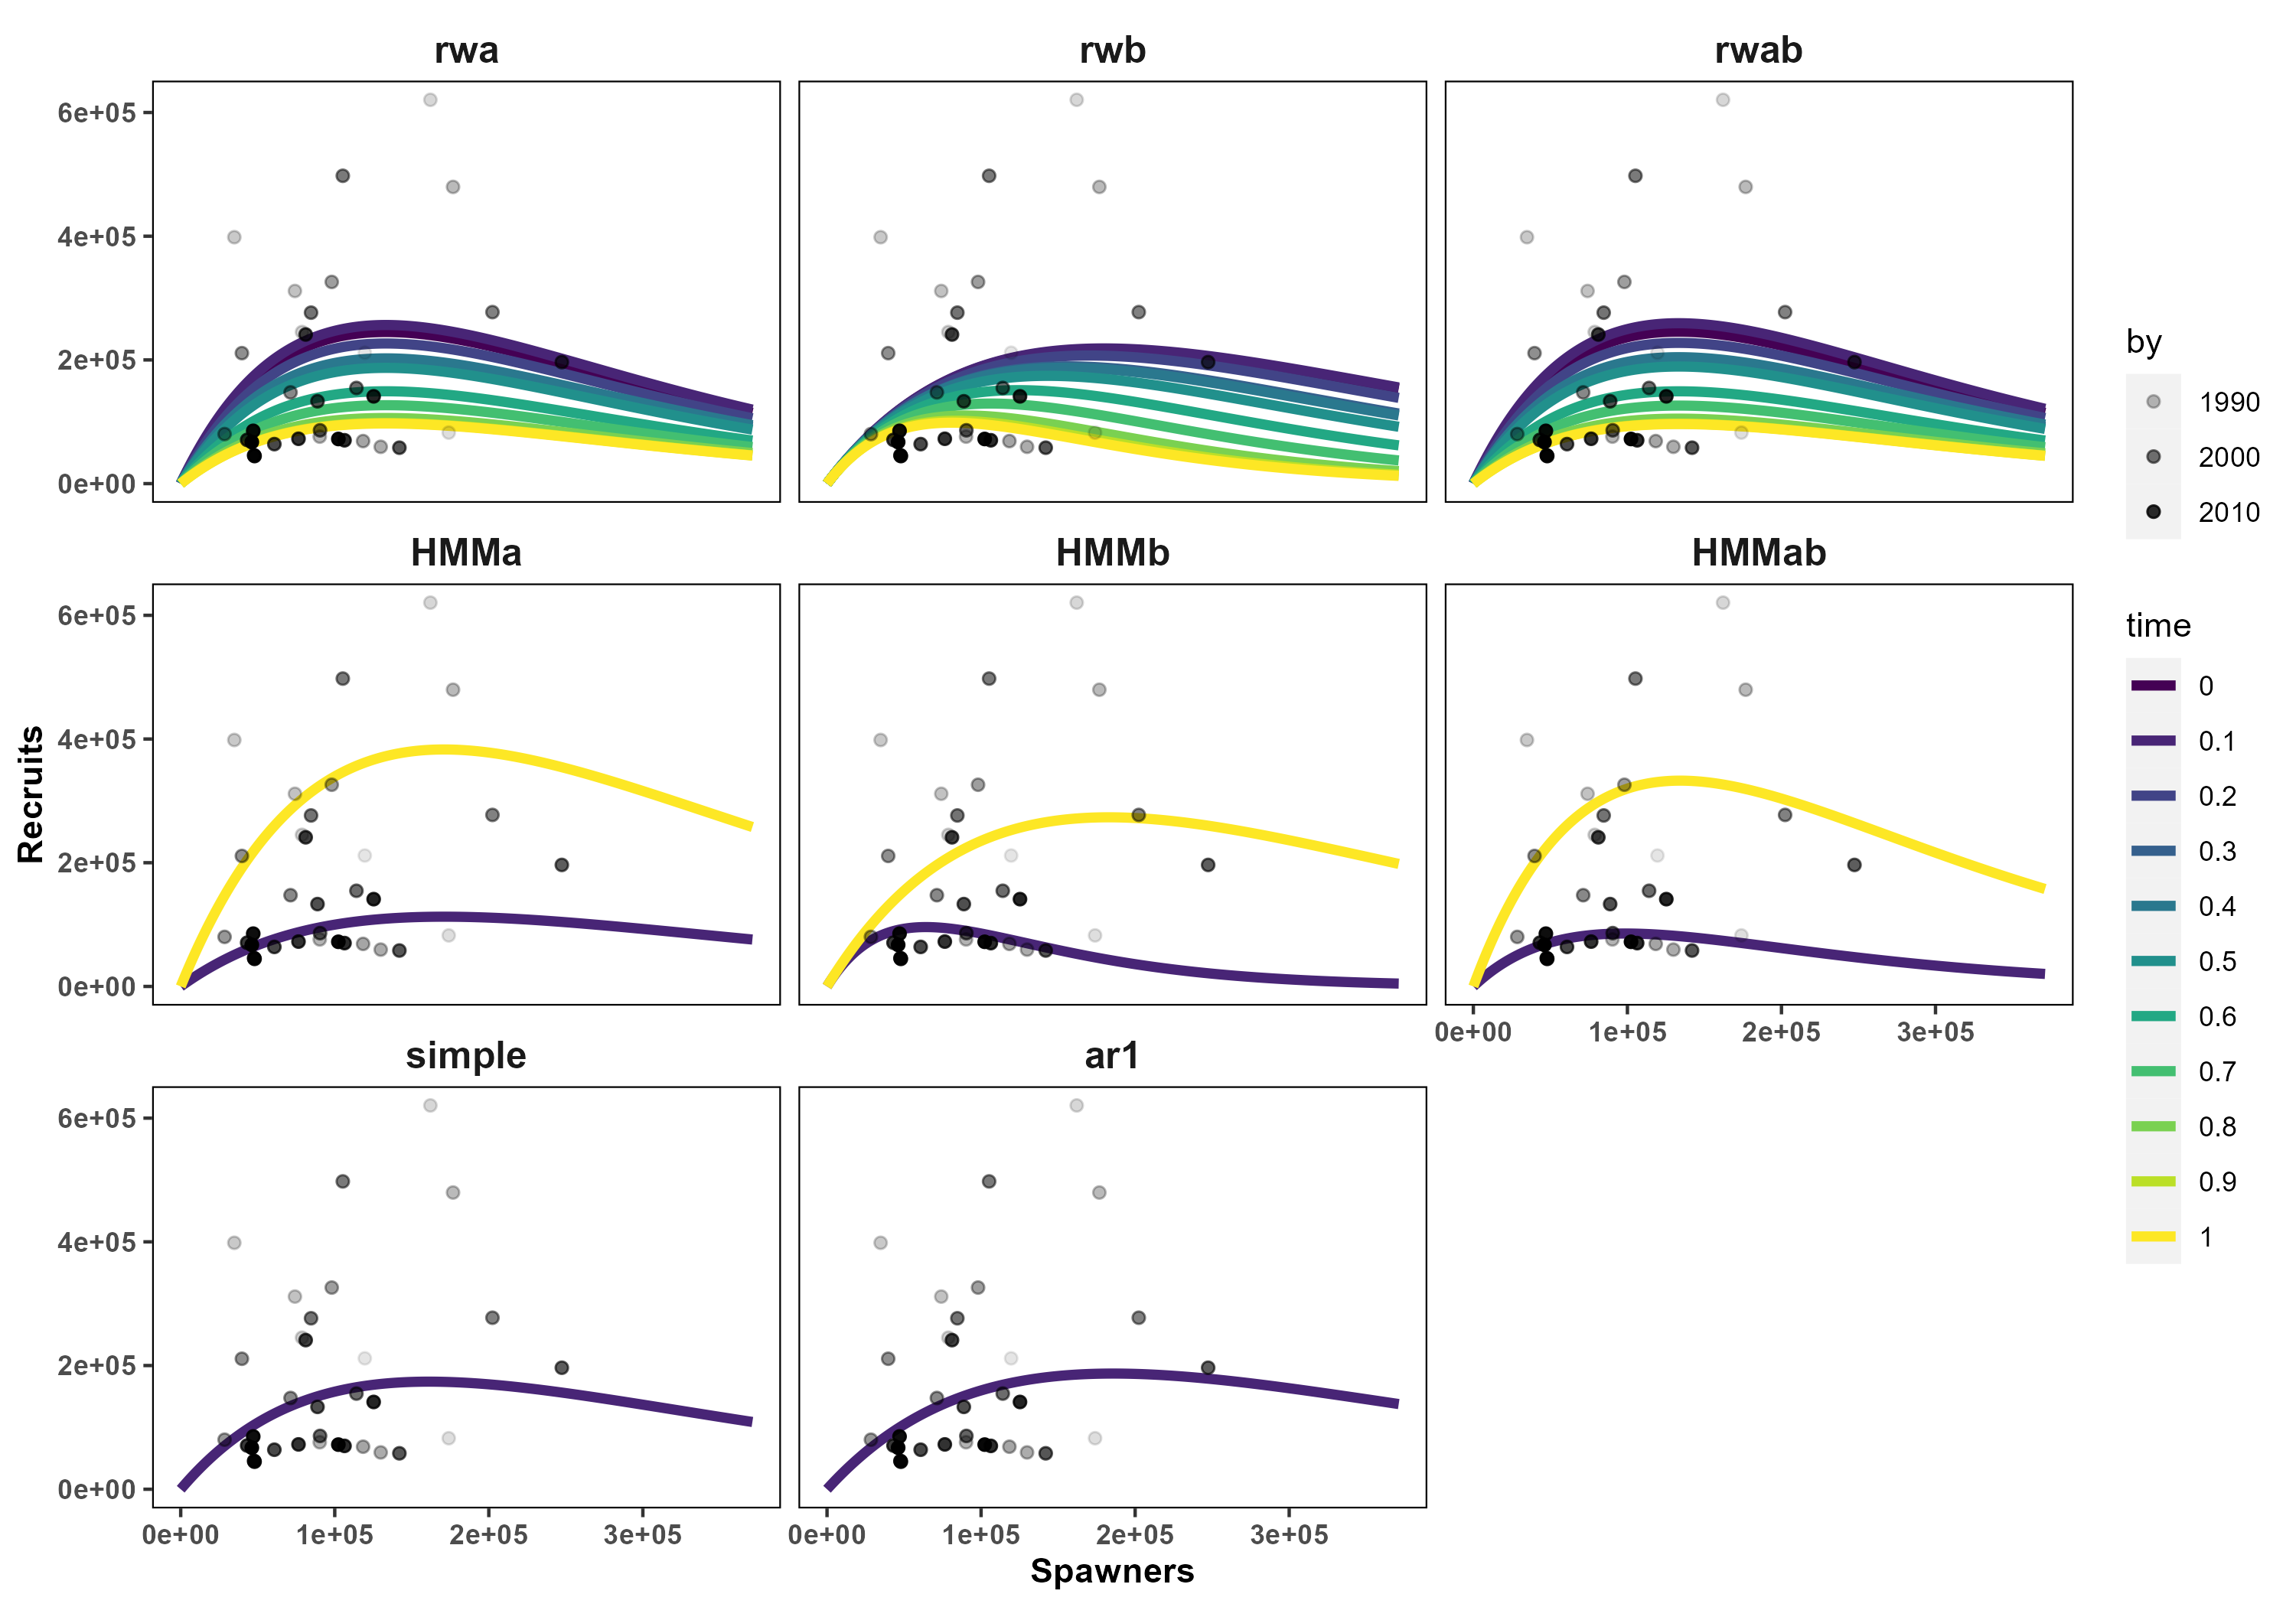
\includegraphics[scale=.52]{predhar.png}
  \caption{Model predictions. Top row indicate random walk models. Middle row regime shift models and bottom row conatin the stationary models with and withour autocorrelated residuals. }
\label{predhar}
\end{figure}




\begin{figure}[htbp]
  \centering
  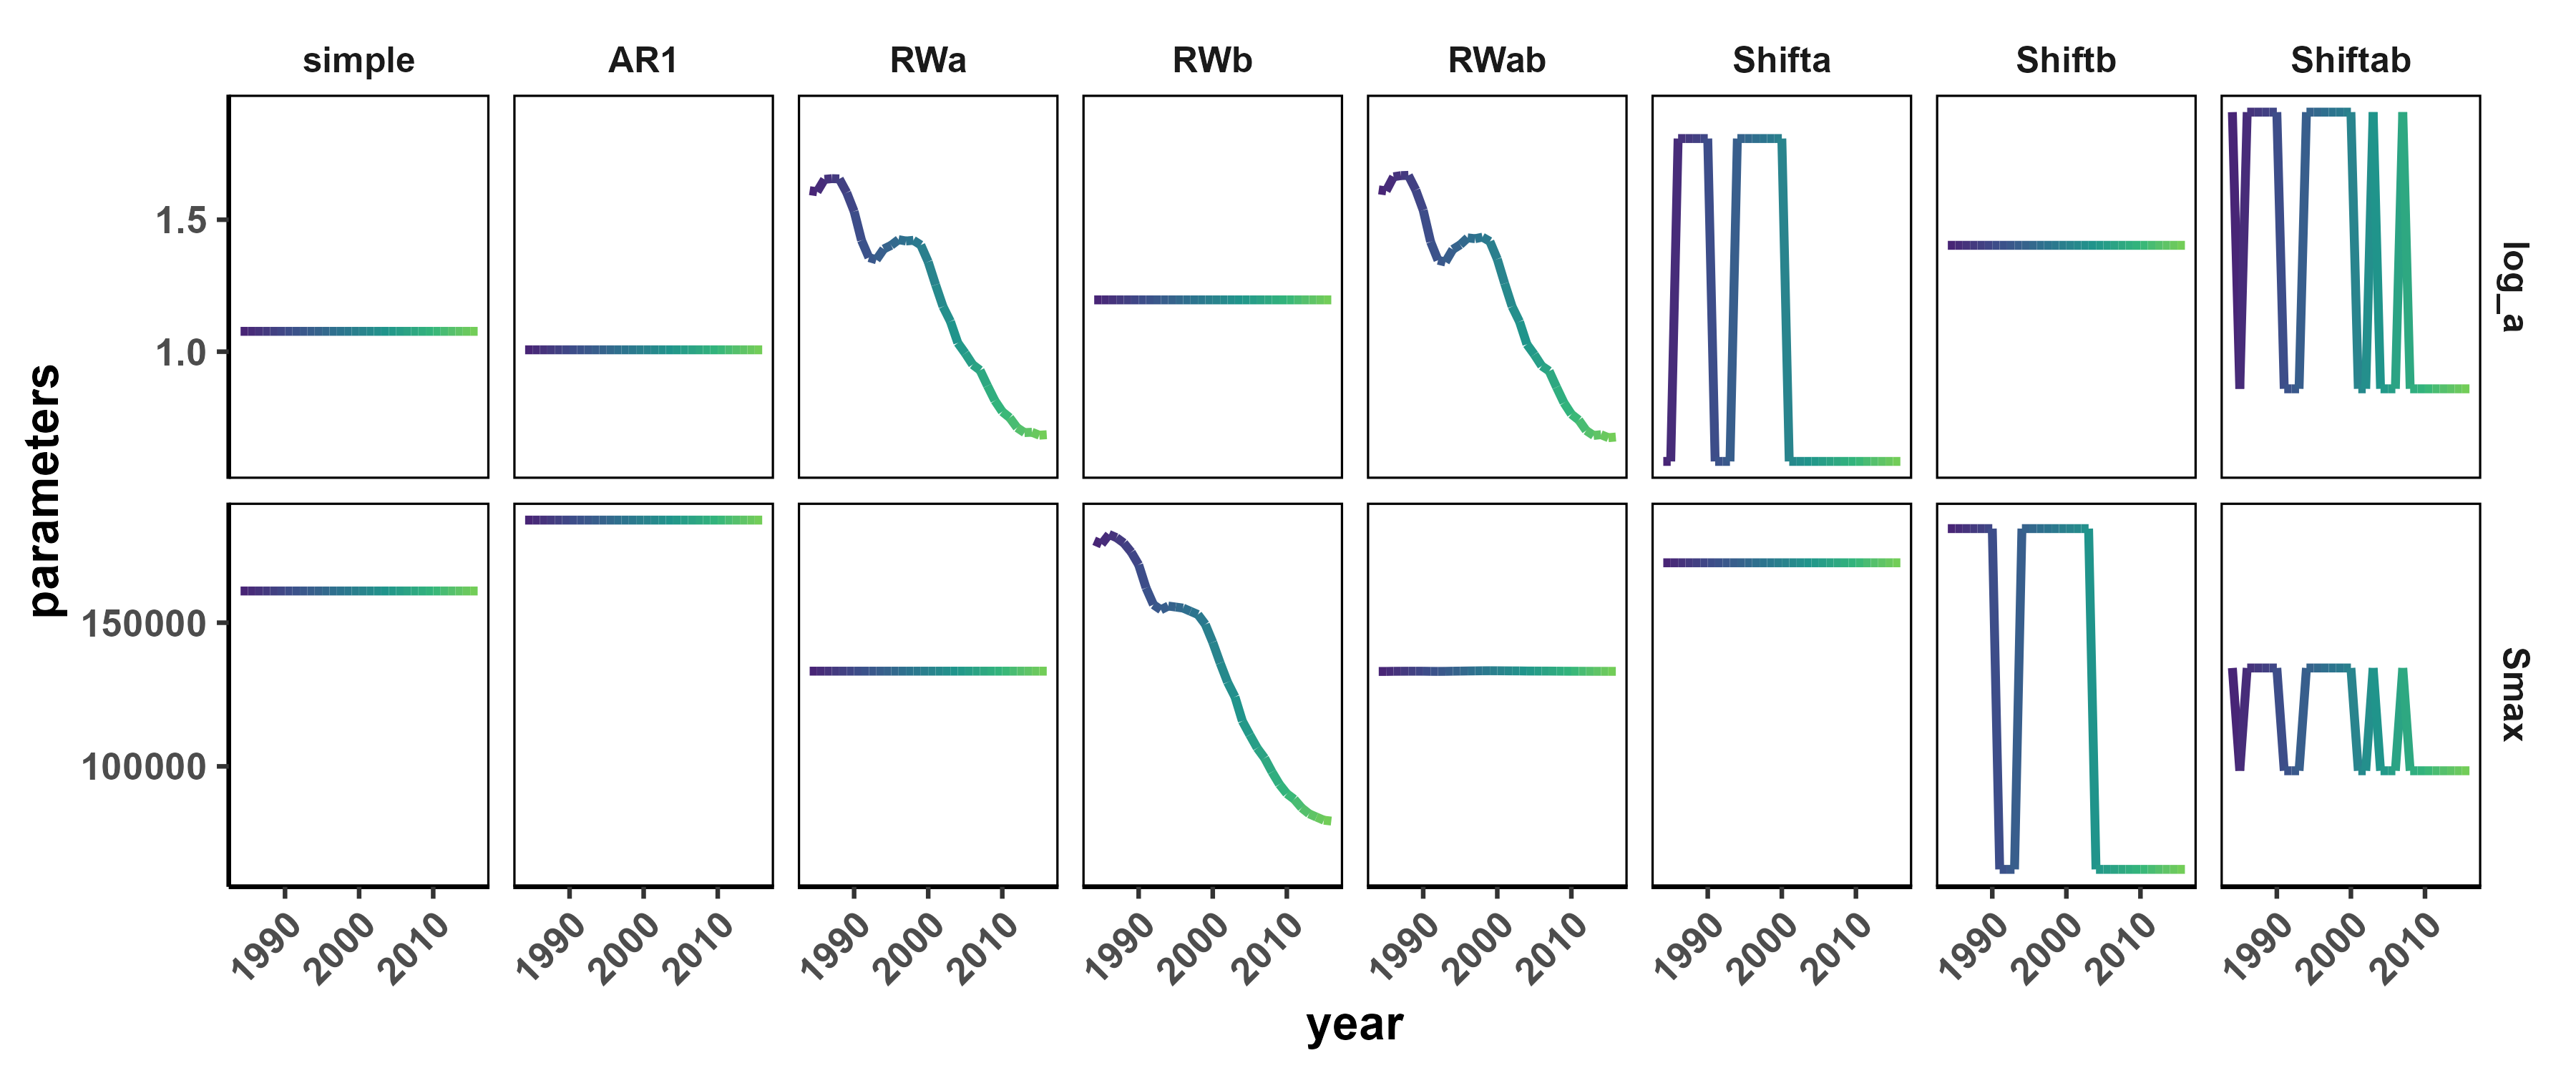
\includegraphics[scale=.52]{paramhar.png}
  \caption{Parameter trajectories for stationary and time varying models considered for Harrison Chinook. }
\label{paramhar}
\end{figure}


\label{seleccrit} 
% latex table generated in R 4.2.1 by xtable 1.8-4 package
% Mon May  1 16:48:01 2023
\begin{table}[ht]
\centering
\caption{Parameter trajectories for stationary 
  and time varying models considered for Harrison Chinook. 
  Minimum AIC and BIC value indicate preferred model, while 
  maximum LFO indicate preferred model. Missing values 
  indicate lack of model convergence} 
\label{harcrit}
\begin{tabular}{rllll}
  \hline
 & model & AIC & BIC & LFO \\ 
  \hline
1 & simple & 11.14 & 10.24 & -20.56 \\ 
  2 & AR1 & 11.05 & 11.05 & \textbf{-19.44} \\ 
  3 & RW a & \textbf{0} & \textbf{0} & - \\ 
  4 & RW b & 7.06 & 7.06 & - \\ 
  5 & RW a and b & - & - & - \\ 
  6 & Shift a & 9.43 & 10.87 & -31.21 \\ 
  7 & Shift b & 19.41 & 20.85 & -38.91 \\ 
  8 & Shift a and b & 14.35 & 15.77 & -42.72 \\ 
   \hline
\end{tabular}
\end{table}



Suggestions of scenarios to be explored for the Harrison stocks in closed-loop simulations:
\begin{samepage}
\begin{itemize}
  \item AR 1 stationary model.
  \item RW a declining trajectory.
  \item RW b declining trajectory (would it be possible?) - could be very interesting ``what if?'' scenario, even if less biologically plausible.
\end{itemize} 
\end{samepage}



\subsection{Cowichan}


Model predictions are in Figure \ref{predcow} and parameter trajectories are in Figure \ref{paramcow}. Model selection criteria are shown in Table \ref{seleccritcow}.



\begin{figure}[htbp]
  \centering
  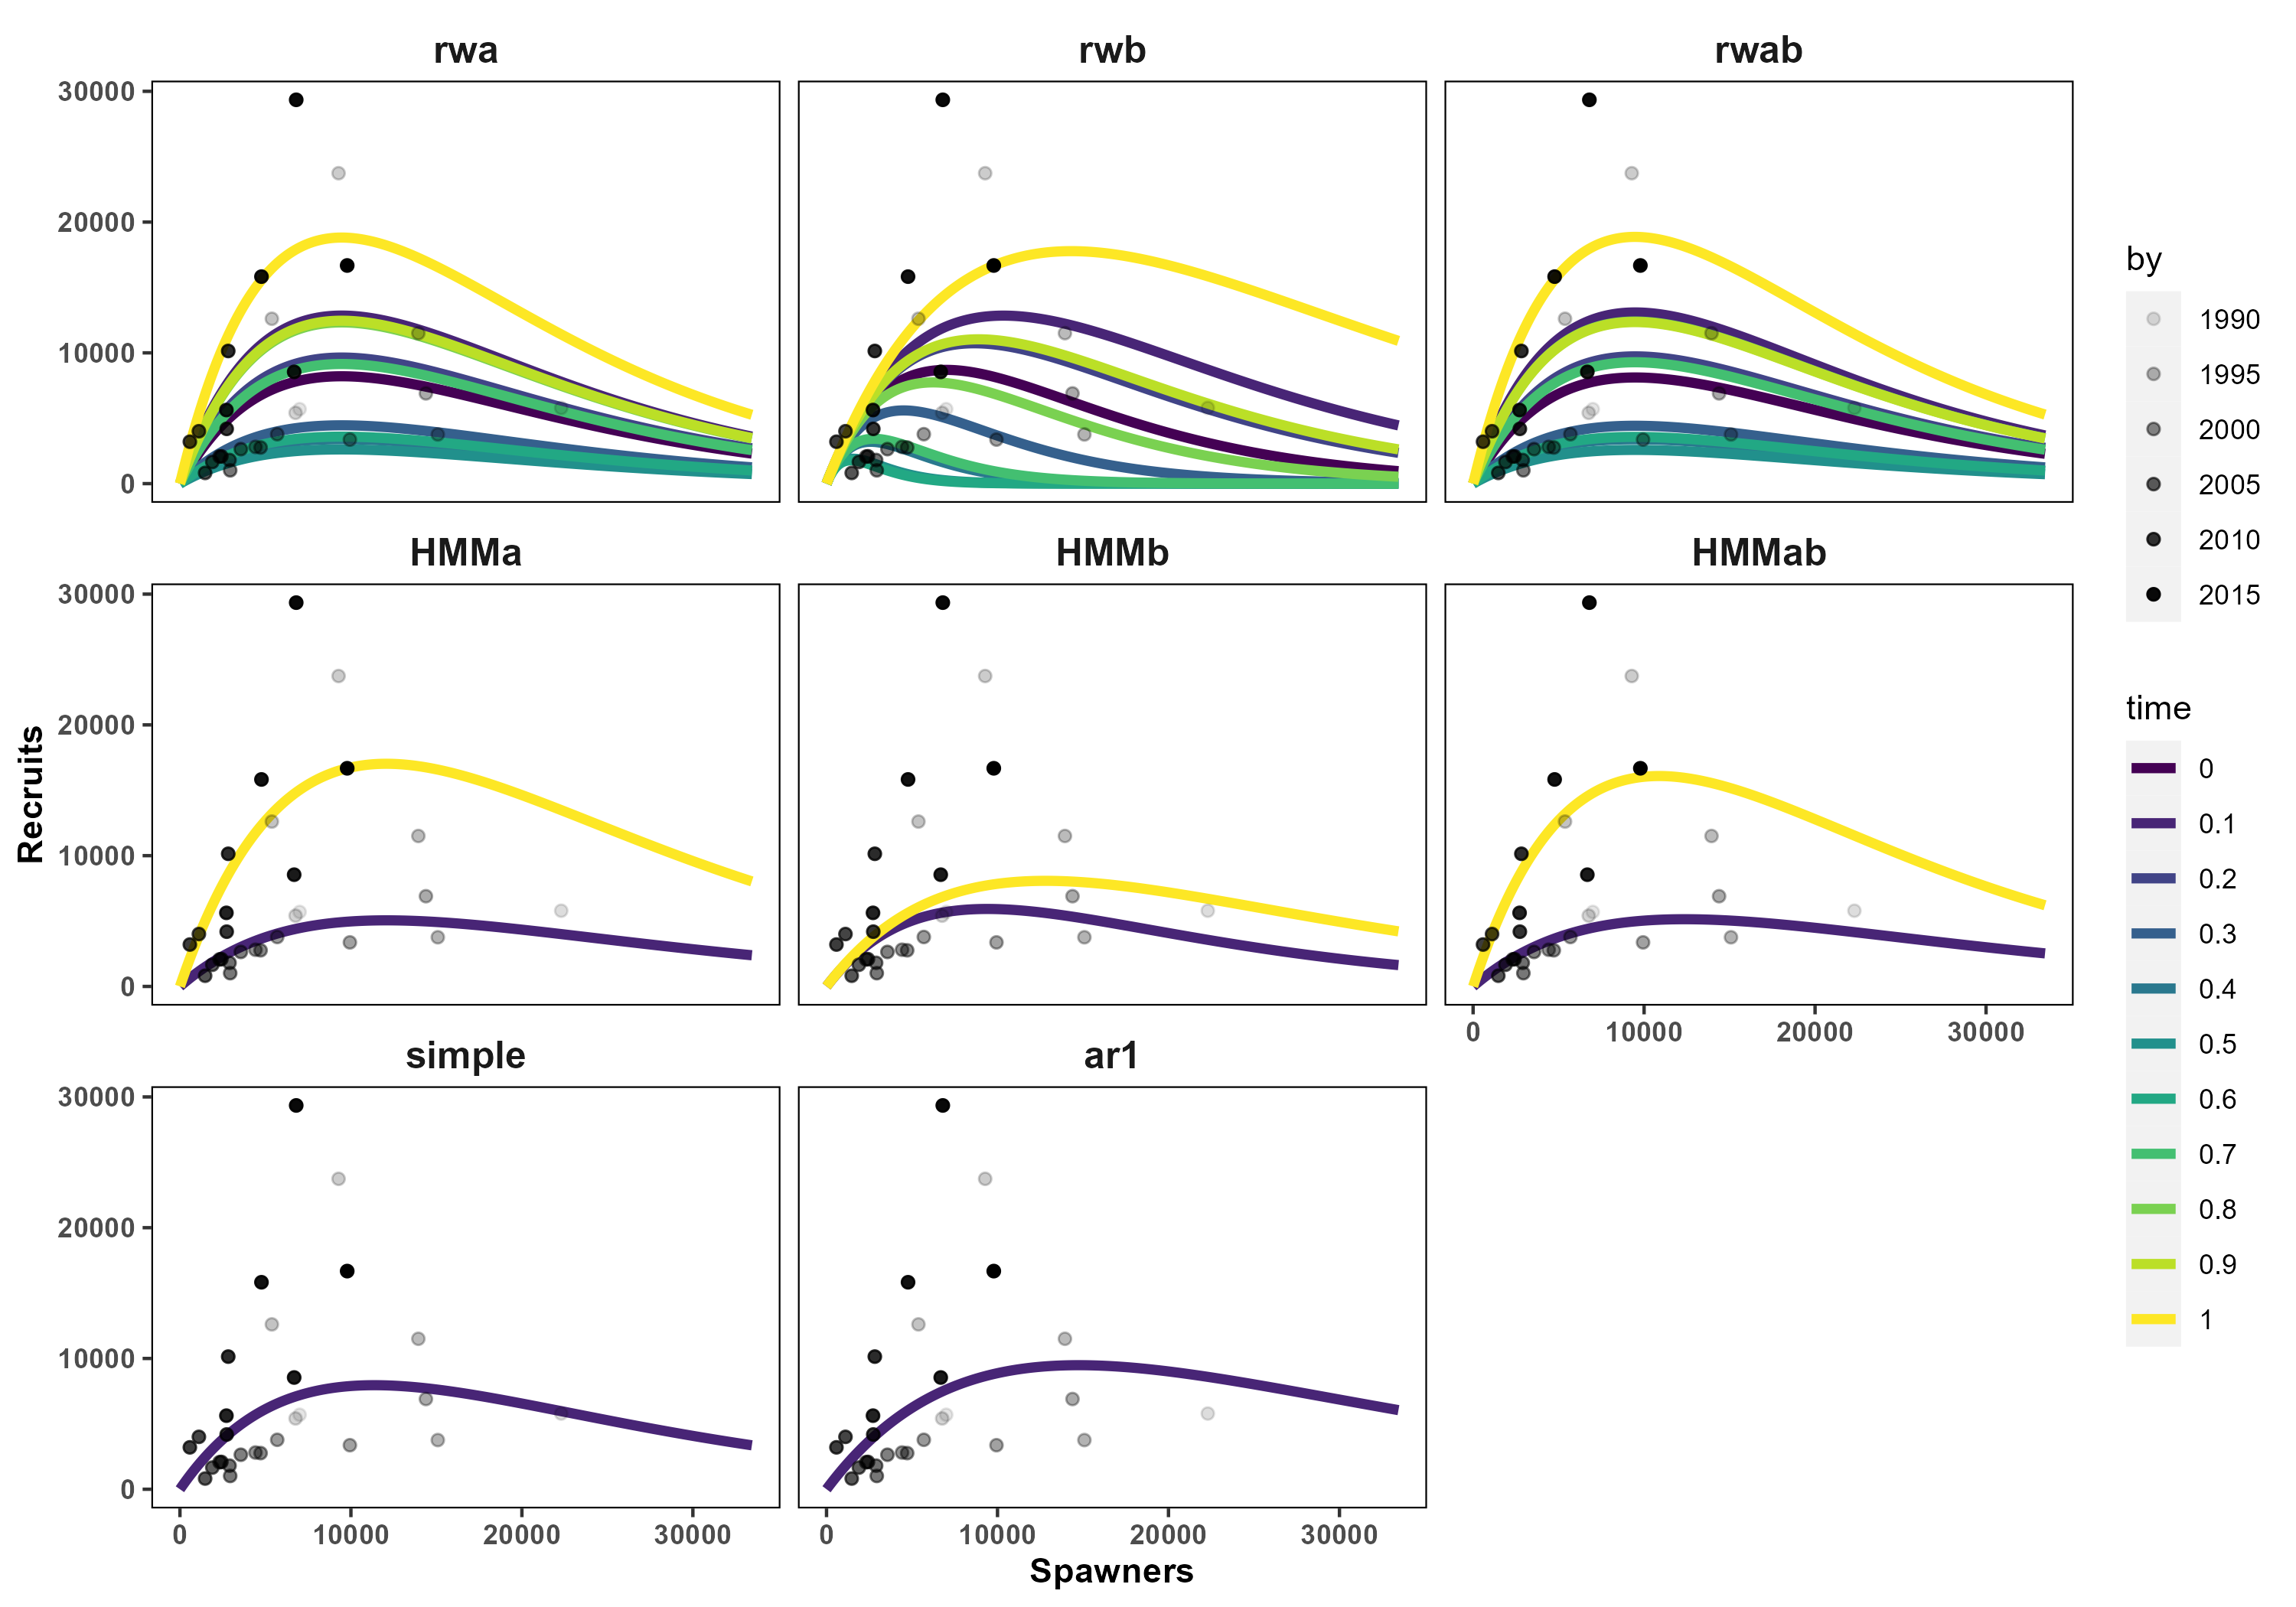
\includegraphics[scale=.52]{predcow.png}
  \caption{Model predictions. Top row indicate random walk models. Middle row regime shift models and bottom row conatin the stationary models with and withour autocorrelated residuals. }
\label{predcow}
\end{figure}




\begin{figure}[htbp]
  \centering
  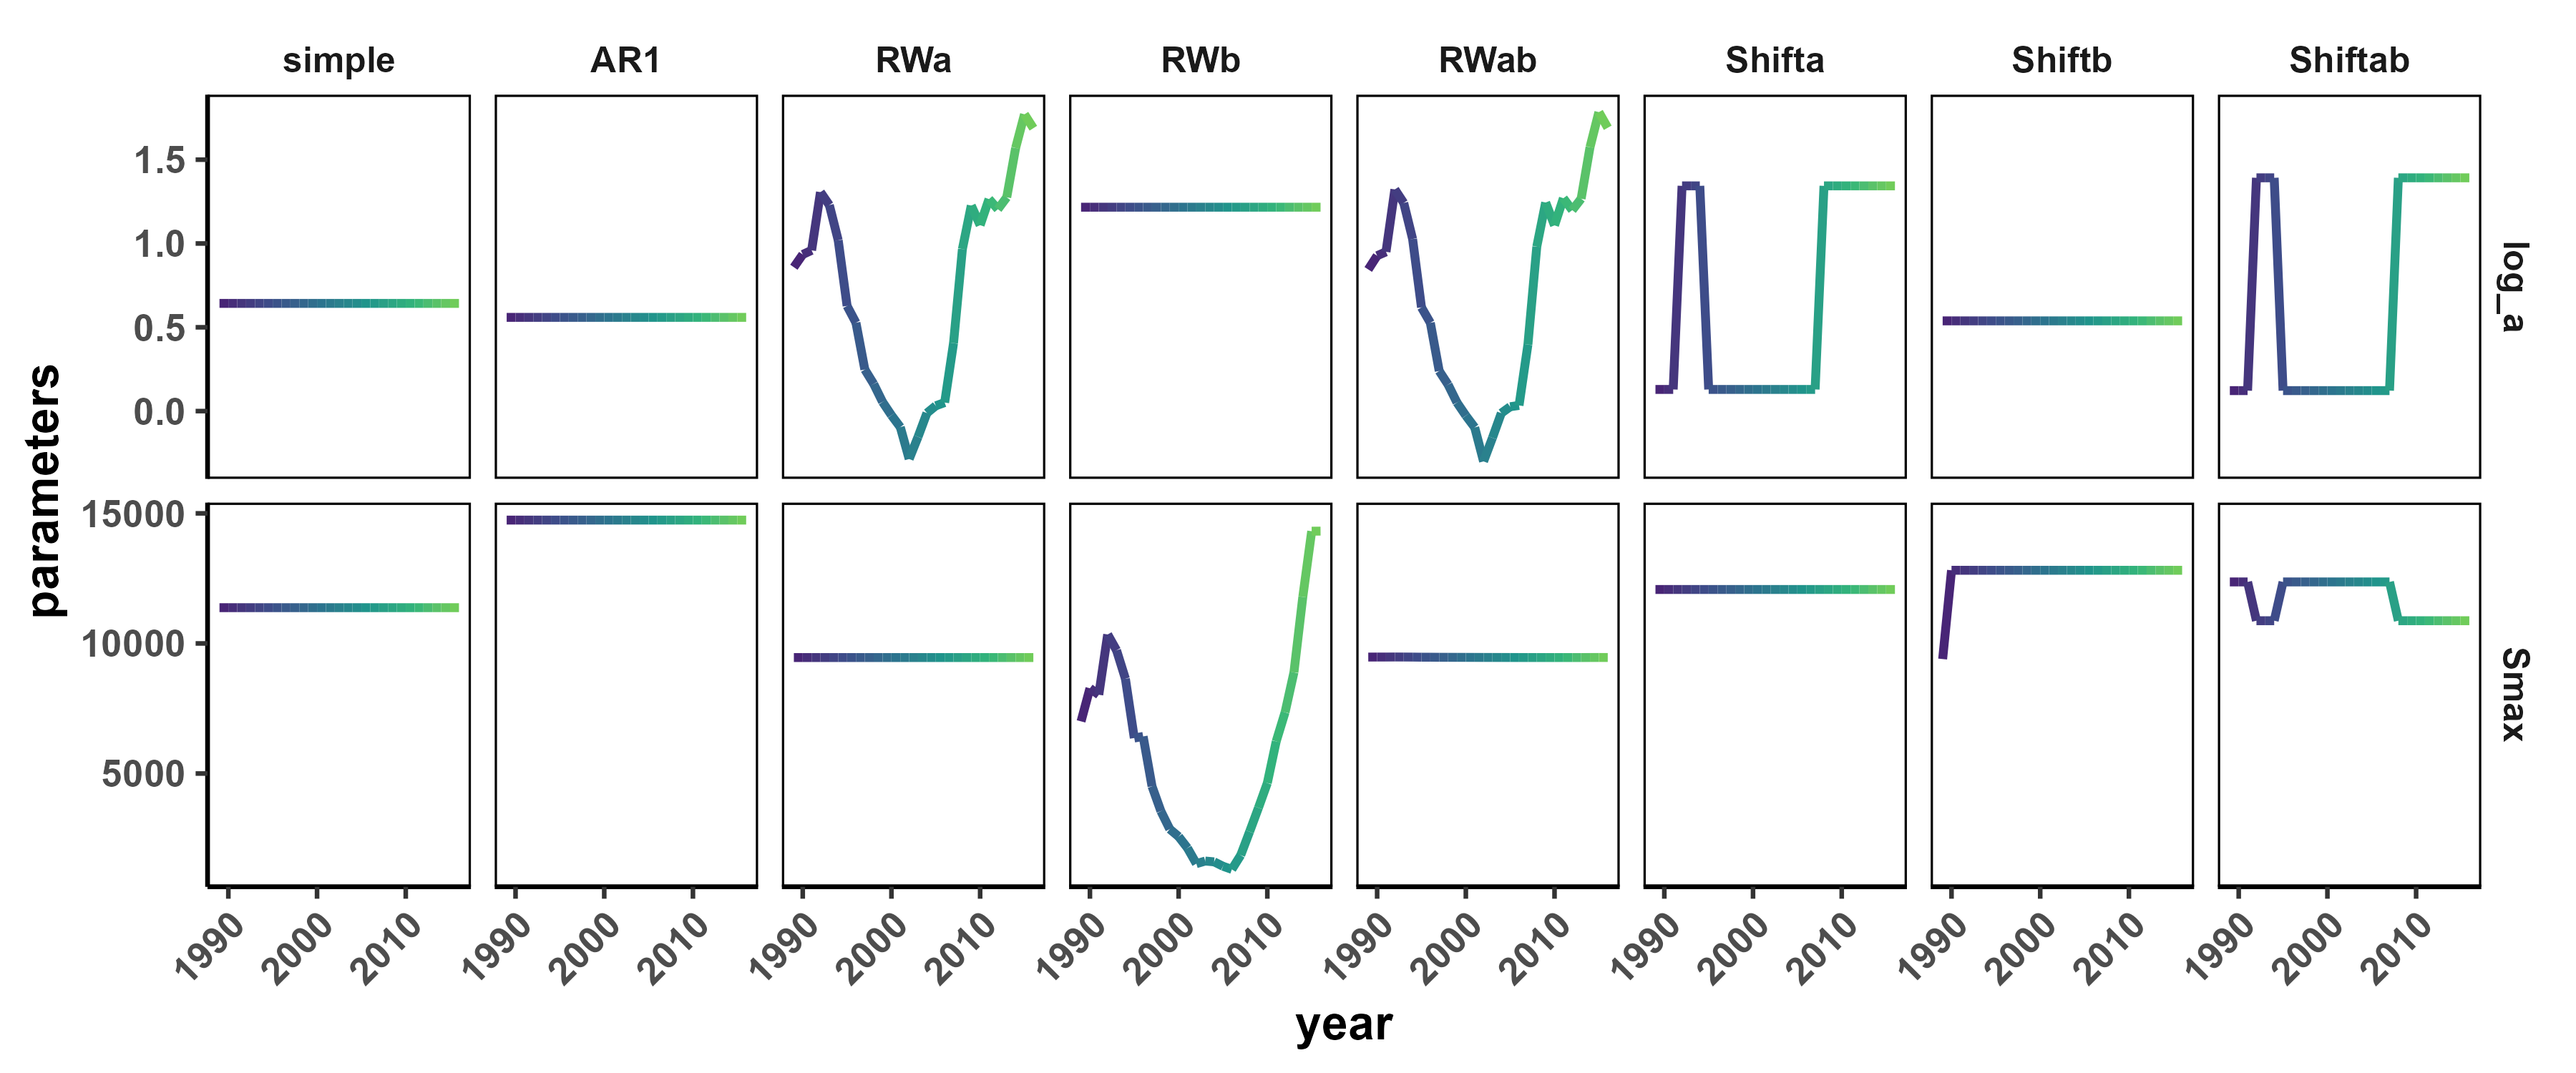
\includegraphics[scale=.52]{paramcow.png}
  \caption{Parameter trajectories for stationary and time varying models considered for Cowichan Chinook. }
\label{paramcow}
\end{figure}


\label{seleccritcow} 
% latex table generated in R 4.2.1 by xtable 1.8-4 package
% Mon May  1 16:47:38 2023
\begin{table}[ht]
\centering
\caption{Parameter trajectories for stationary 
  and time varying models considered for Cowichan Chinook. Minimum 
  AIC and BIC value indicate preferred model, while maximum LFO indicate 
  preferred model. Missing values indicate lack of model convergence} 
\label{cowcrit}
\begin{tabular}{rllll}
  \hline
 & model & AIC & BIC & LFO \\ 
  \hline
1 & simple & 43.74 & 43.15 & - \\ 
  2 & AR1 & 36.44 & 36.44 & - \\ 
  3 & RW a & \textbf{0} & \textbf{0} & -21.13 \\ 
  4 & RW b & 6.37 & 6.37 & -18.07 \\ 
  5 & RW a and b & 1.5 & 1.84 & \textbf{-17.44} \\ 
  6 & Shift a & 35.64 & 35.78 & - \\ 
  7 & Shift b & - & - & -20.08 \\ 
  8 & Shift a and b & 39.33 & 38.82 & -22.56 \\ 
   \hline
\end{tabular}
\end{table}





Suggestions of scenarios to be explored for the Cowichan stocks in closed-loop simulations:
\begin{samepage}
\begin{itemize}
  \item stationary model.
  \item Shift a  trajectory.
  \item RW b declining trajectory (?).
\end{itemize} 
\end{samepage}
%\bibliographystyle{apa} 
%\bibliography{report.bib}


\end{document}





%fn+control+alt+del for clean up!
